\documentclass[tikz,border=10pt]{standalone}
\usepackage{tkz-euclide} % 基于TikZ，专门用于几何绘图

\begin{document}

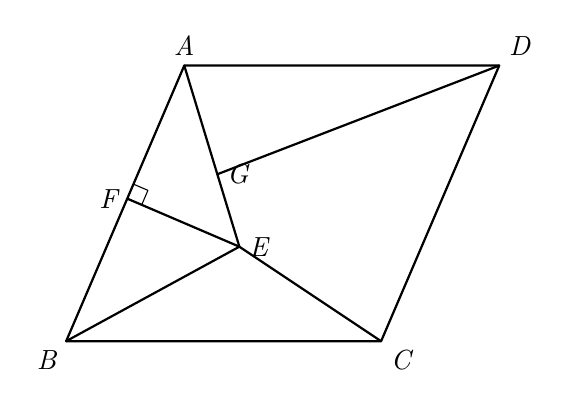
\begin{tikzpicture}[line cap=round, line join=round, >=stealth, font=\itshape]
    % --- 1. 定义核心顶点坐标 ---
    % 定义平行四边形 A, B, C, D
    \coordinate (B) at (0, 0);
    \coordinate (C) at (4, 0);
    \coordinate (A) at (1.5, 3.5);
    \coordinate (D) at ($(A)+(C)-(B)$); % 平行向量计算 D 点

    % --- 2. 内部点位计算 ---
    % E 点位于对角线/中线区域，根据视觉比例取在 AC 附近
    \coordinate (E) at (2.2, 1.2);

    % F 点在 AB 上，且满足 EF \perp AB (垂足)
    \coordinate (F) at ($(A)!(E)!(B)$);

    % G 点在 AE 上
    \coordinate (G) at ($(A)!0.6!(E)$);

    % --- 3. 绘制主体连线 ---
    % 绘制外围平行四边形
    \draw[thick] (A) -- (B) -- (C) -- (D) -- cycle;

    % 绘制内部连线
    \draw[thick] (A) -- (E);
    \draw[thick] (B) -- (E);
    \draw[thick] (C) -- (E);
    \draw[thick] (D) -- (G);
    \draw[thick] (E) -- (F);

    % --- 4. 绘制直角标记 ---
    % 在 F 点标注直角 (EFB = 90度)
    \tkzMarkRightAngle[size=0.2](E,F,A)

    % --- 5. 标注字母标签 ---
    \node[above] at (A) {A};
    \node[below left] at (B) {B};
    \node[below right] at (C) {C};
    \node[above right] at (D) {D};
    \node[right] at (E) {E};
    \node[left] at (F) {F};
    \node[right] at (G) {G};

\end{tikzpicture}

\end{document}